\documentclass[a4paper,12pt]{article}

\usepackage[utf8]{inputenc}
\usepackage[T1]{fontenc}
\usepackage[ngerman]{babel}
\usepackage{hyperref}
\usepackage{graphicx}
\usepackage{geometry}
\geometry{margin=2.5cm}

\title{Konzeptabgabe}
\date{}

\begin{document}

\maketitle

\noindent\textbf{Themenbereich:} LLM Performance Vergleich (Feature Realisation) \\
\textbf{Werkzeug:} \href{https://github.com/TobiasKiecker/CASCADE}{CASCADE} \\
\textbf{Gruppenmitglieder:} Bruno Vincent Hemoura, Alexander Hristov, Caspar Moritz Klein \\
\textbf{Gruppe:} 01

% -------------------------------------------------------
\section{Forschungsfrage}

Wie kann CASCADE so erweitert werden,
dass LLM-Nutzung, Laufzeitverhalten und Resultate der Pipeline
strukturiert erfasst werden,
um verschiedene Modelle, Prompts und Ausführungsschritte
vergleichbar zu machen?

% -------------------------------------------------------
\section{Abstract}

CASCADE generiert und validiert Tests mithilfe einer mehrstufigen Pipeline
aus Extraktion, Analyse, Generierung und Ausführung.
Für einen fundierten LLM-Performance-Vergleich fehlte bisher
eine zentrale Erfassung von Tokenverbrauch, Laufzeiten und Fehlern.
Im Rahmen dieser Feature-Realisierung wird ein leichtgewichtiger
Metrics-Mechanismus für CASCADE implementiert.
Er soll Events wie bestimmmte Utility-Aufrufe order Fehler protokollieren und
am Ende eines Runs eine Zusammenfassung generiere.
Besonders liegt der Fokus auf LLM-Aufrufen sowie zentralen Pipeline-Schritten.
Das bisherige Loggging von Fehlern soll dabei ausgebaut werden,
sodass Schwachstellen und Zeitverluste einfacher zu erkennen sind.

Mit der erfolgten Implementierung werden wir den Mechanismus
anhand verschiedener Modelle demonstrieren.

% -------------------------------------------------------
\section{Motivation}

LLM-basierte Test- und Codegenerierung ist stark abhängig von
Modell, Prompting, Eingabegröße und Ausführungsumgebung.
Ohne einheitliche Metriken ist schwer nachvollziehbar,
ob ein Modell tatsächlich bessere Ergebnisse liefert
oder nur höhere Kosten bzw.\ längere Laufzeiten verursacht.
Ziel ist daher eine reproduzierbare Messgrundlage,
mit der Tokenverbrauch, Dauer, Fehler und zentrale Teilschritte
der CASCADE-Pipeline objektiv verglichen werden können.

Bisher ist schwer zu erkennen, wann Fehler passieren und welche Ursachen diese haben.
Es gibt keine einheitliche Konvention, wie Fehler ausgegeben werden,
wodurch vorallem in den Komponenten zur Generation,
Fehler schwer einzuordnen sind.
Deshalb ist die Erweiterung des Loggings auch sinnvoll,
weil CASCADE dadurch nicht nur Endergebnisse,
sondern auch deren Entstehung nachvollziehbar macht.
So können Unterschiede zwischen Modellen oder Konfigurationen
später anhand konkreter Messwerte statt nur anhand
beobachteter Resultate bewertet werden.

% -------------------------------------------------------
\section{Lösungsansatz}

Vorgesehen ist ein leichtgewichtiges Metrics-Konzept,
das pro CASCADE-Run strukturierte Ereignisse erfasst
und anschließend aggregierte Kennzahlen bereitstellt.
Dabei sollen sowohl LLM-spezifische Daten
wie Input-, Output- und Total-Tokens
als auch allgemeine Performance-Daten
wie Laufzeit, Fehler und Pipeline-Phase berücksichtigt werden.

Die Erfassung soll möglichst nah an den relevanten Pipeline-Schritten ansetzen,
ohne die bestehende CASCADE-Architektur stark zu verändern.
Sinnvoll ist eine Kombination aus expliziten Events
für fachliche Informationen
und Zeitmessungen für größere Ausführungsblöcke.
Kontextinformationen wie Phase, Methode oder Sample
sollen automatisch mitgeführt werden,
damit die Messdaten später einem konkreten Pipeline-Schritt
zugeordnet werden können.

Es sollen Pipeline-weite Hilfsfunktionen eingeführt werden,
welche von allen Komponenten genutzt werden können um
Events wie Fehler, Info-Nachrichten, LLM-Nutzungen oder
Zeitverbrauche einheitlich in die gemeinsame Messung
einzutragen, welche am Ende des Runs zusammengefasst wird.

% -------------------------------------------------------
\section{Skizze}

\begin{figure}[h]
    \centering
    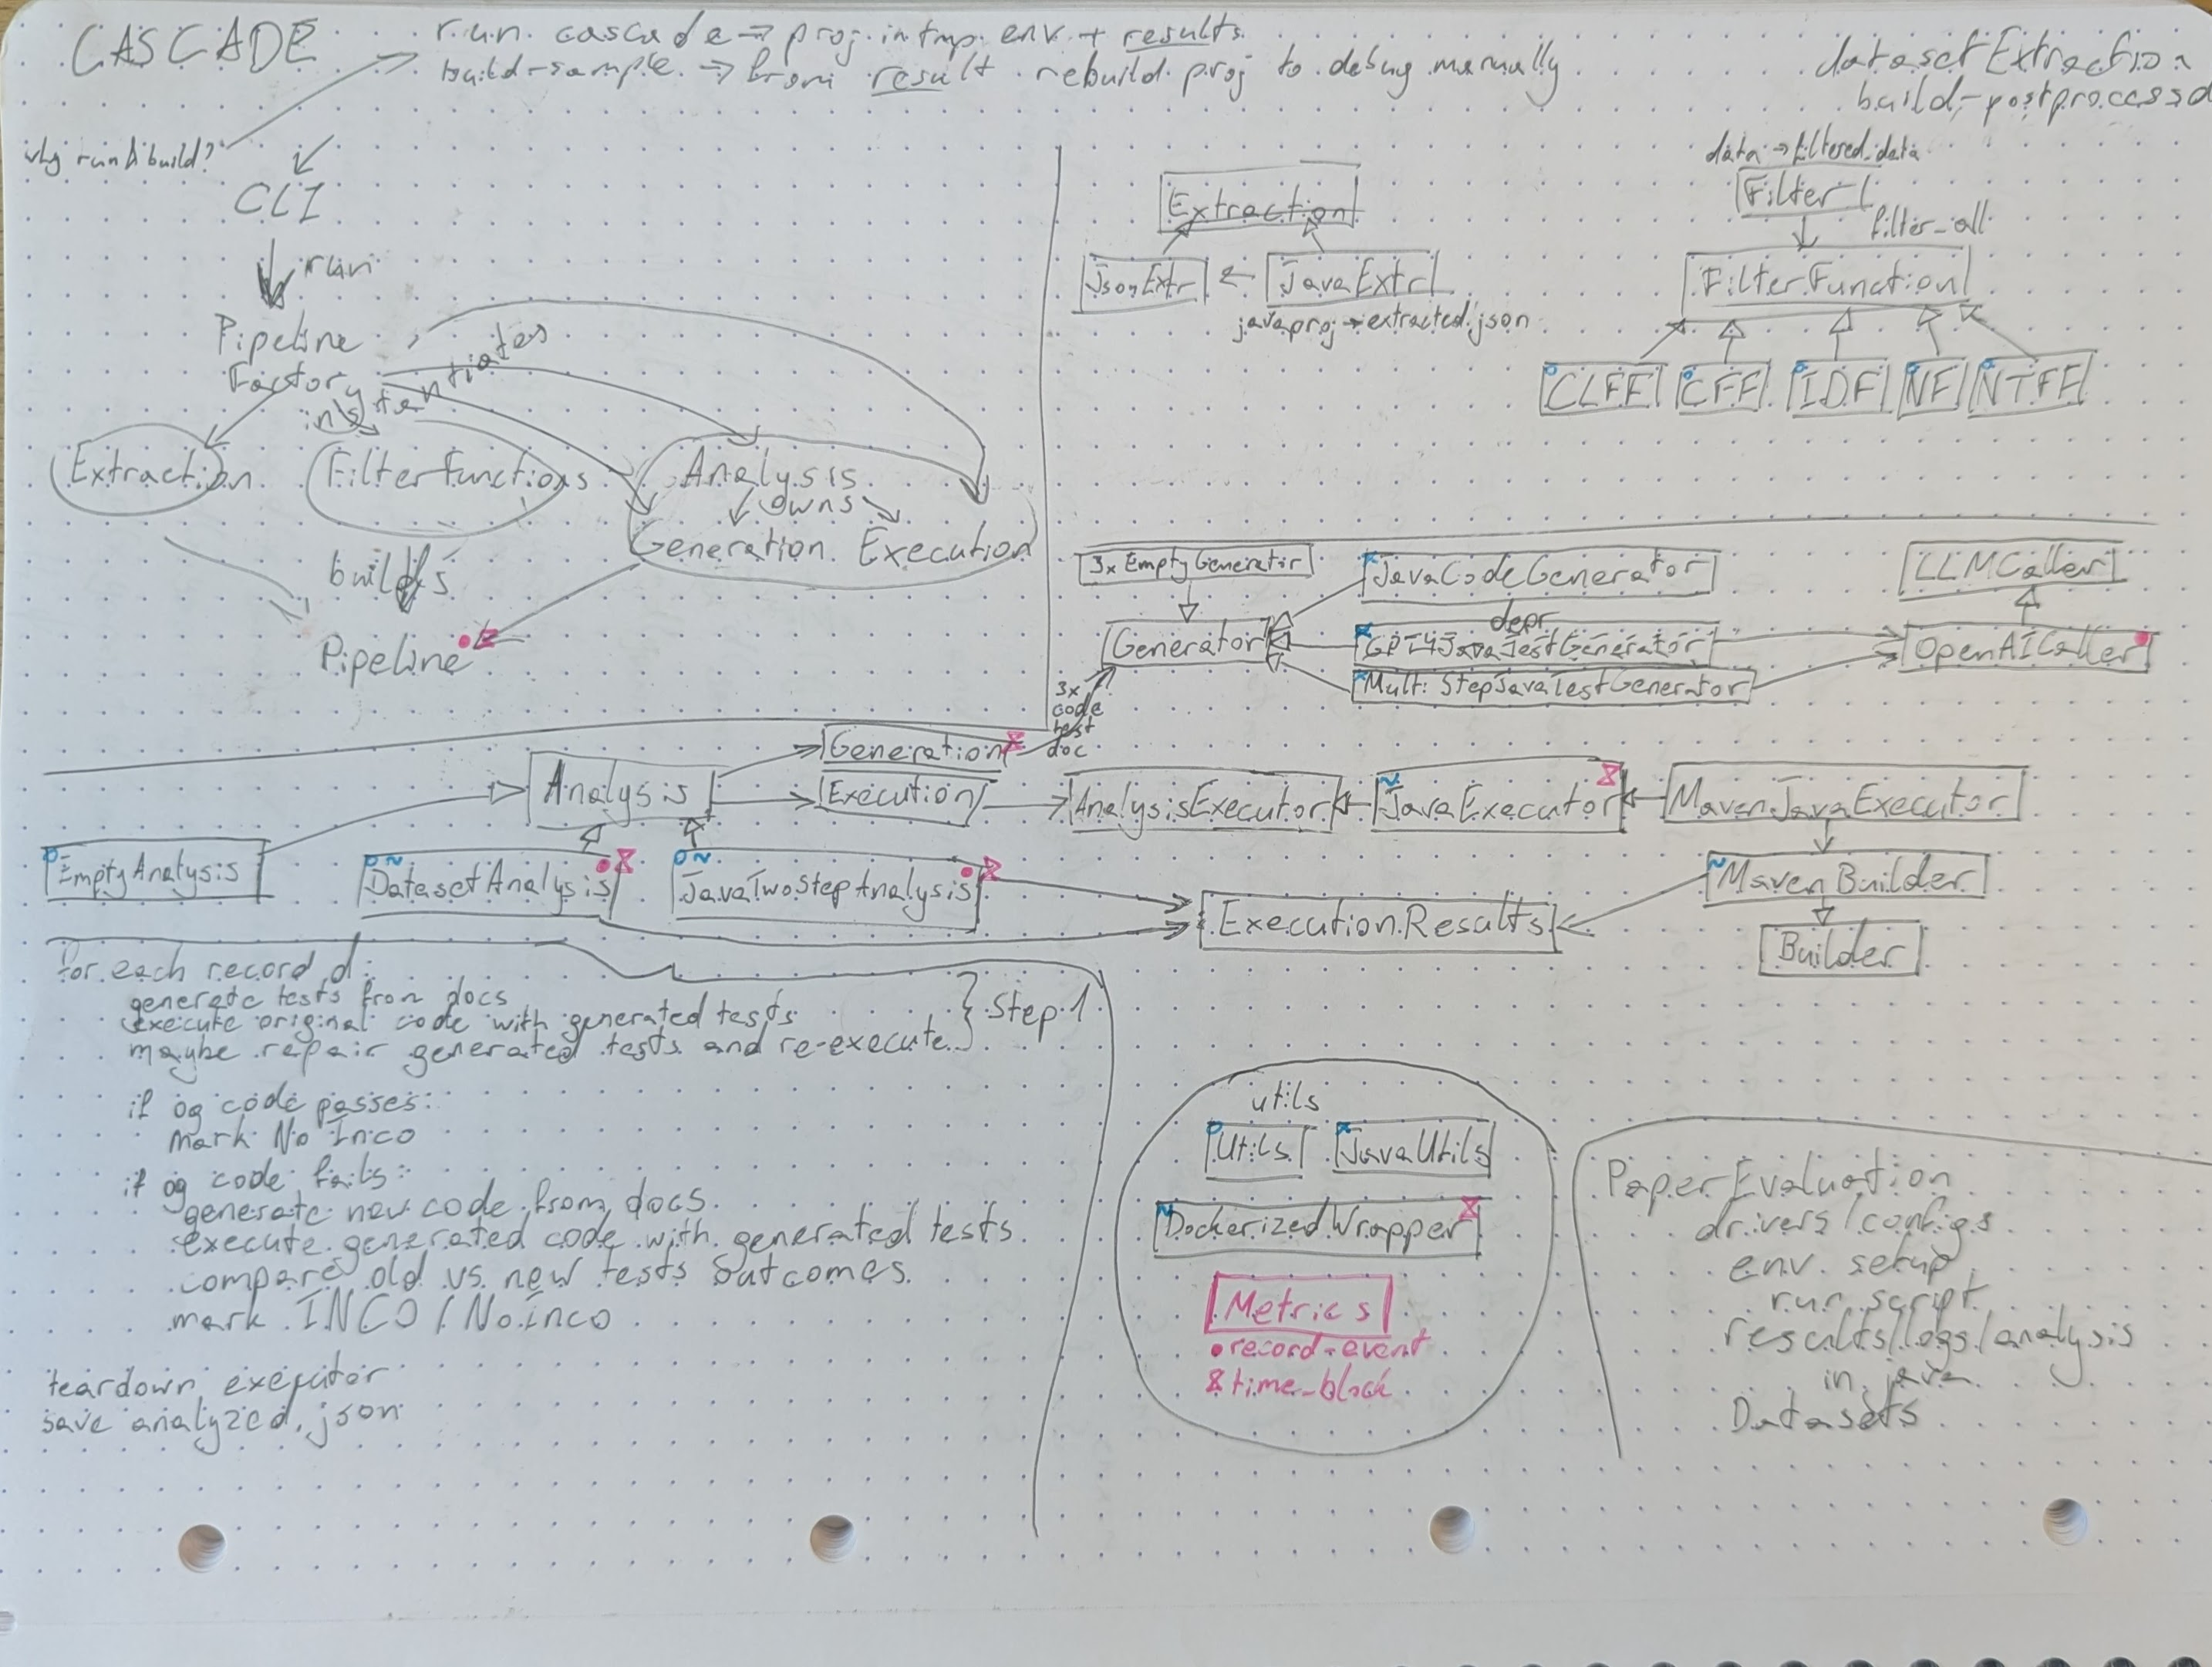
\includegraphics[width=0.8\textwidth]{imgs/PXL_20260616_170314467.MP.jpg}
    \caption{Skizze der Pipeline-Architektur}
\end{figure}

\end{document}
